\subsection{Profile and roofline}\label{sec:profile}

With the numerical target and its limiting error established, the discussion now turns to the hardware cost of producing it.

At $n=61$, the system has 226{,}981 unknowns, 4.23M nonzeros, and ${\approx}49$\,MB in compressed sparse column form. Over 100 time steps, SpMV and Gram--Schmidt dominate the KSM-EI solve, while the dense $\exp(\mat{H}_m)$ is marginal (\Cref{tab:profile}). Gram--Schmidt's share grows with the grid because the Krylov dimension $m$ grows and MGS is quadratic in $m$. The \emph{other} column contains vector updates, endpoint-defect norm computations, and per-time-step bookkeeping outside the three instrumented kernels.

\begin{table}[htbp!]
\centering
\caption{Kernel shares of KSM-EI solve time (basket, tolerance $10^{-8}$). $\bar m$ is the
mean Krylov dimension; \emph{other} is uninstrumented work (vector updates, error
estimation, bookkeeping).}
\label{tab:profile}
\begin{tabular}{@{}lccccc@{}}
\toprule
\textbf{Grid} & $\bar{m}$ & \textbf{SpMV} & \textbf{Gram--Schmidt} & \textbf{dense expm} & \textbf{other} \\
\midrule
$n=31$ & 7.60 & 82.9\% & 11.7\% & 0.40\% & 4.9\% \\
$n=53$ & 8.42 & 77.7\% & 16.8\% & 0.34\% & 5.1\% \\
$n=65$ & 9.24 & 76.0\% & 18.0\% & 0.21\% & 5.9\% \\
$n=73$ & 9.89 & 75.2\% & 18.8\% & 0.15\% & 5.9\% \\
$n=89$ & 11.34 & 70.3\% & 23.8\% & 0.08\% & 5.8\% \\
\bottomrule
\end{tabular}
\end{table}

Both kernels remain far below the compute ceiling. The cache-aware roofline explains why and locates the CA opportunity (\Cref{fig:roofline}) \cite{williams-2009}. Puffin's measured single-core roofs are 20.9\,GB/s for DRAM, 58.2\,GB/s for L3, 88.6\,GB/s for L2, and 68.1\,GFLOP/s for an FMA compute loop.

\begin{figure}[t!]
\centering
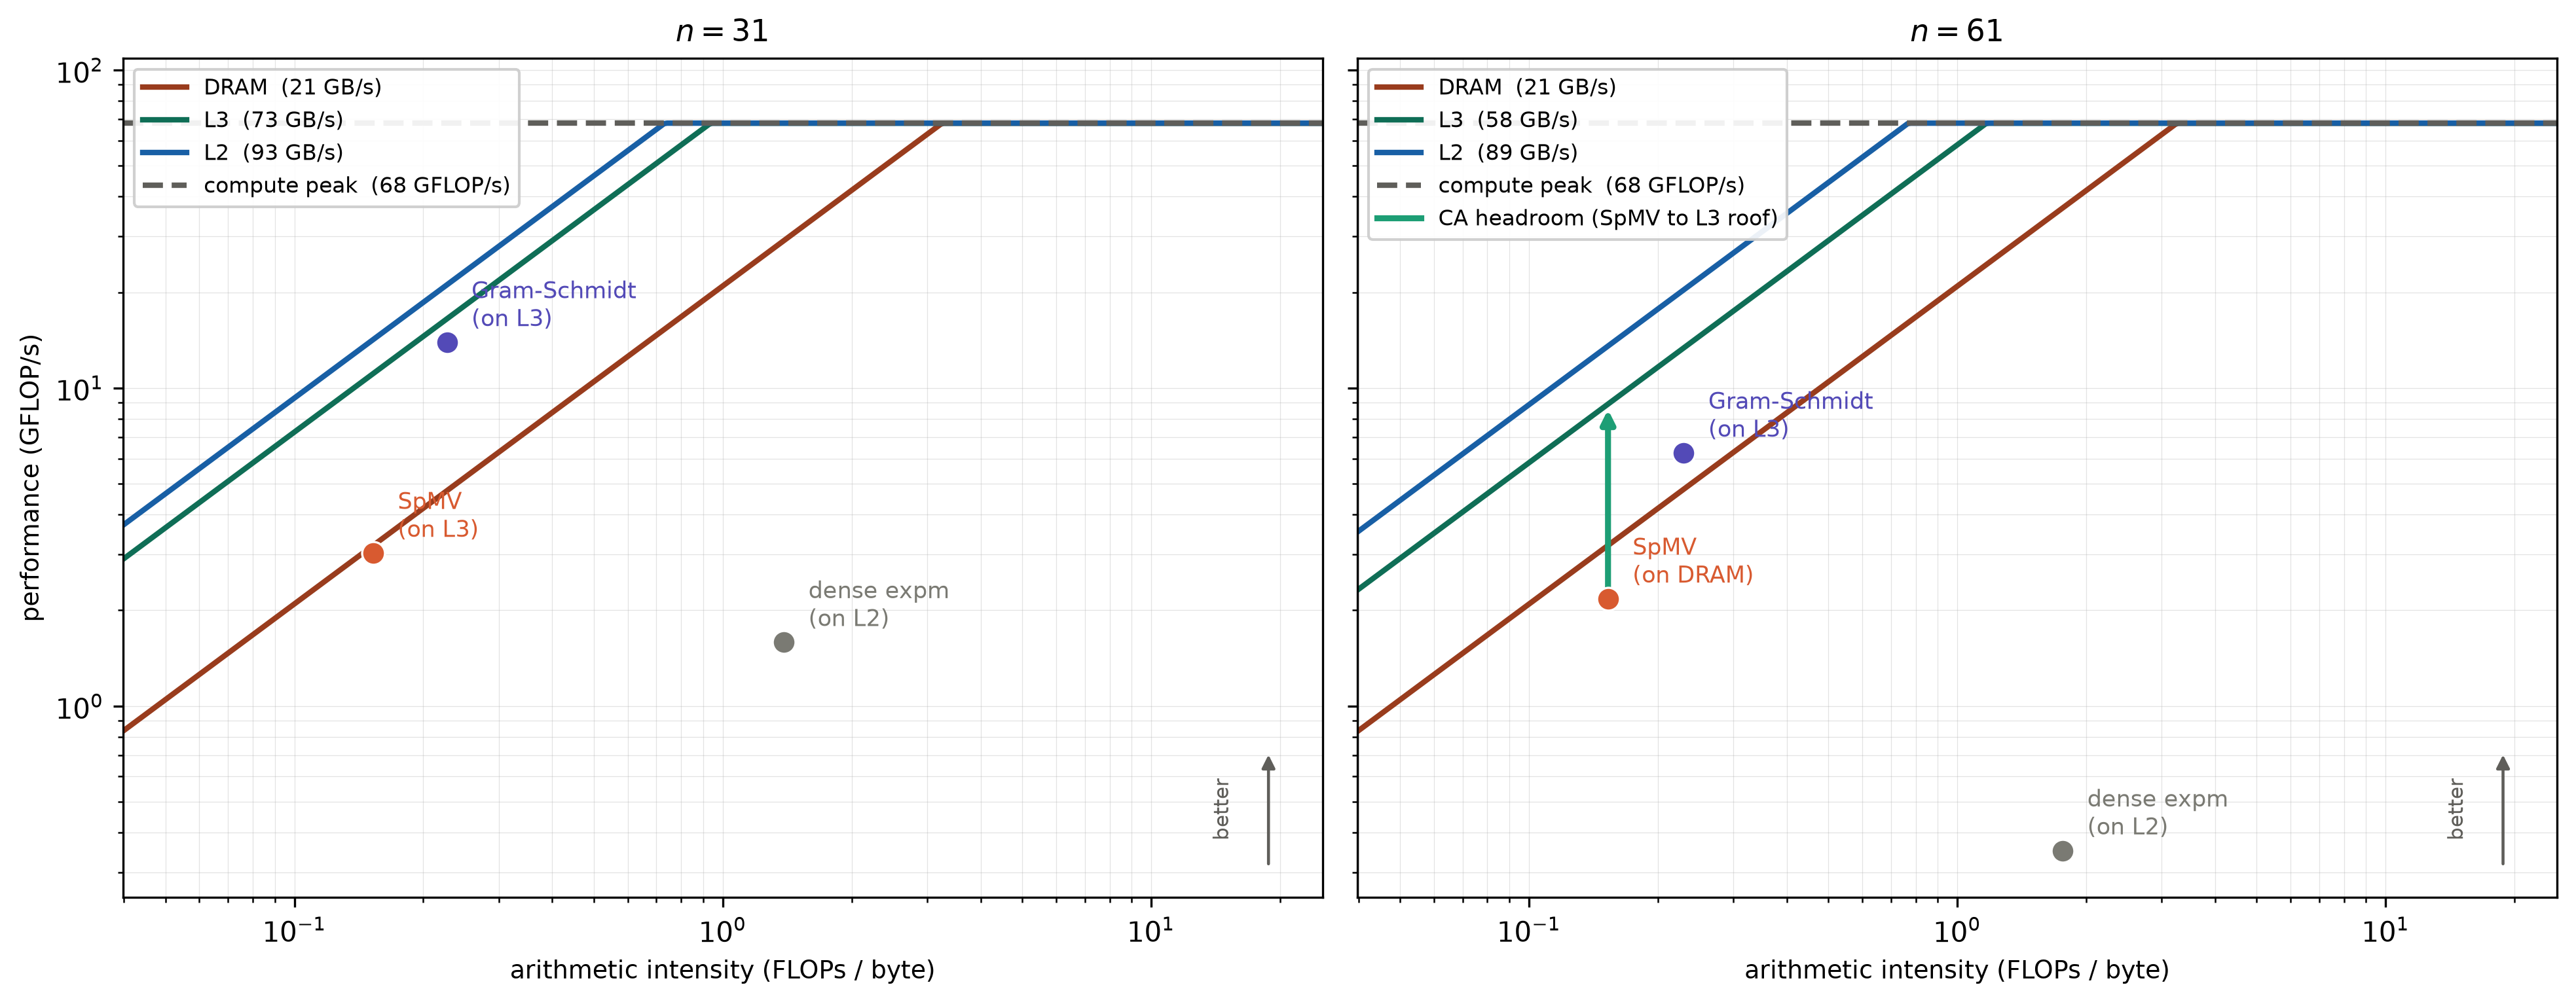
\includegraphics[width=0.72\textwidth]{cache_roofline.png}
\caption{Cache-aware roofline for the two hot kernels at $n=31$ and $n=61$. At $n=61$ the SpMV has spilled to DRAM, the vertical distance from the measured point to the L3 roof at the same arithmetic intensity is exactly the traffic a matrix-powers reformulation would recover.}
\label{fig:roofline}
\end{figure}

The attainable gain from moving a kernel one tier up the hierarchy is
\begin{equation}
\text{gain} = \frac{\min(BW_{\text{fast}} \cdot AI,\ \text{peak})} {\min(BW_{\text{slow}} \cdot AI,\ \text{peak})},
\label{eq:gain}
\end{equation}
This expression becomes the bandwidth ratio only while \emph{both} roofs remain sloped. Once the fast roof reaches the compute ceiling, the gain bends downward. A matrix-powers kernel can reach this point because its arithmetic intensity is approximately $s\times$ higher.
